\input{../../../headers/tpheaders.tex}

\prob{Étudier le comportement d'un redresseur} \\

\graphicspath{{../../../img/}}
\begin{center}
\def\svgwidth{\columnwidth}
\input{../../../img/triptyque.pdf_tex}
\end{center}

\section{Étude des schémas}

Le destructeur d'aiguilles nécessite une alimentation en énergie électrique pour fonctionner.

Afin d'alimenter les circuits électroniques de commande et de puissance, il est nécessaire de fournir respectivement des tensions d'alimentation $+5\,\text{V}$ et $+24\,\text{V}$.

La tension $+5\,\text{V}$ alimentant les circuits de commande doit être parfaitement continue alors que les circuits de puissance seront alimentés sous un courant simplement filtré.

L'alimentation du destructeur d'aiguilles peut se représenter comme sur la figure \ref{fig01}.

\begin{figure}[!ht]
\begin{center}
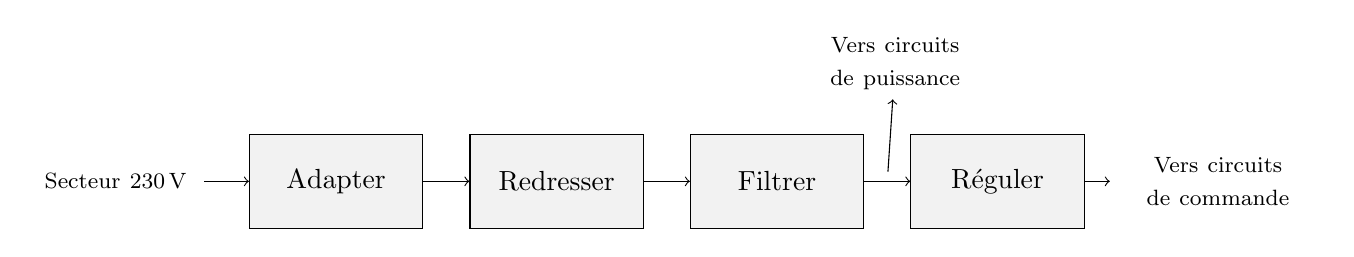
\begin{tikzpicture}[node distance=1.8cm, auto,
  block/.style={rectangle, draw, text centered, minimum height=1.2cm, minimum width=2.2cm, fill=gray!10}]
  \node[text width=2cm, align=center] (entree)
    {\footnotesize Secteur 230\,V};
  \node [block, right of=entree, node distance=2.8cm] (adapt)   {Adapter};
  \node [block, right of=adapt, node distance=2.8cm] (redress) {Redresser};
  \node [block, right of=redress, node distance=2.8cm] (filtre)  {Filtrer};
  \node [right of=filtre, node distance=1.4cm] (connec)  {};
  \node [right of=filtre, node distance=1cm, above of=filtre, node distance=1.5cm, text width=2.5cm, align=center] (puiss)   {\footnotesize Vers circuits de puissance};
  \node [block, right of=filtre, node distance=2.8cm] (regul)   {Réguler};
 \node [right of=regul, node distance=2.8cm, text width=2.5cm, align=center] (comma)   {\footnotesize Vers circuits de commande};
 
  \draw[->] (adapt)   -- (redress);
  \draw[->] (redress) -- (filtre);
  \draw[->] (filtre)  -- (regul);
  \draw[->] (entree)   -- (adapt);
  \draw[->] (connec)   -- (puiss);
  \draw[->] (regul)   -- (comma);

\end{tikzpicture}
\end{center}
\caption{Schéma fonctionnel de la fonction Alimenter}
\label{fig01}
\end{figure}

Dans la platine alimentation, on abaisse le secteur 230\,V à une valeur de 32\,V grâce à un transformateur. Puis on redresse ce signal à l'aide d'un pont de diodes. 

Vient ensuite le filtrage avec condensateur puis la régulation par le biais d'un circuit intégré.

\begin{figure}[!ht]
\begin{center}
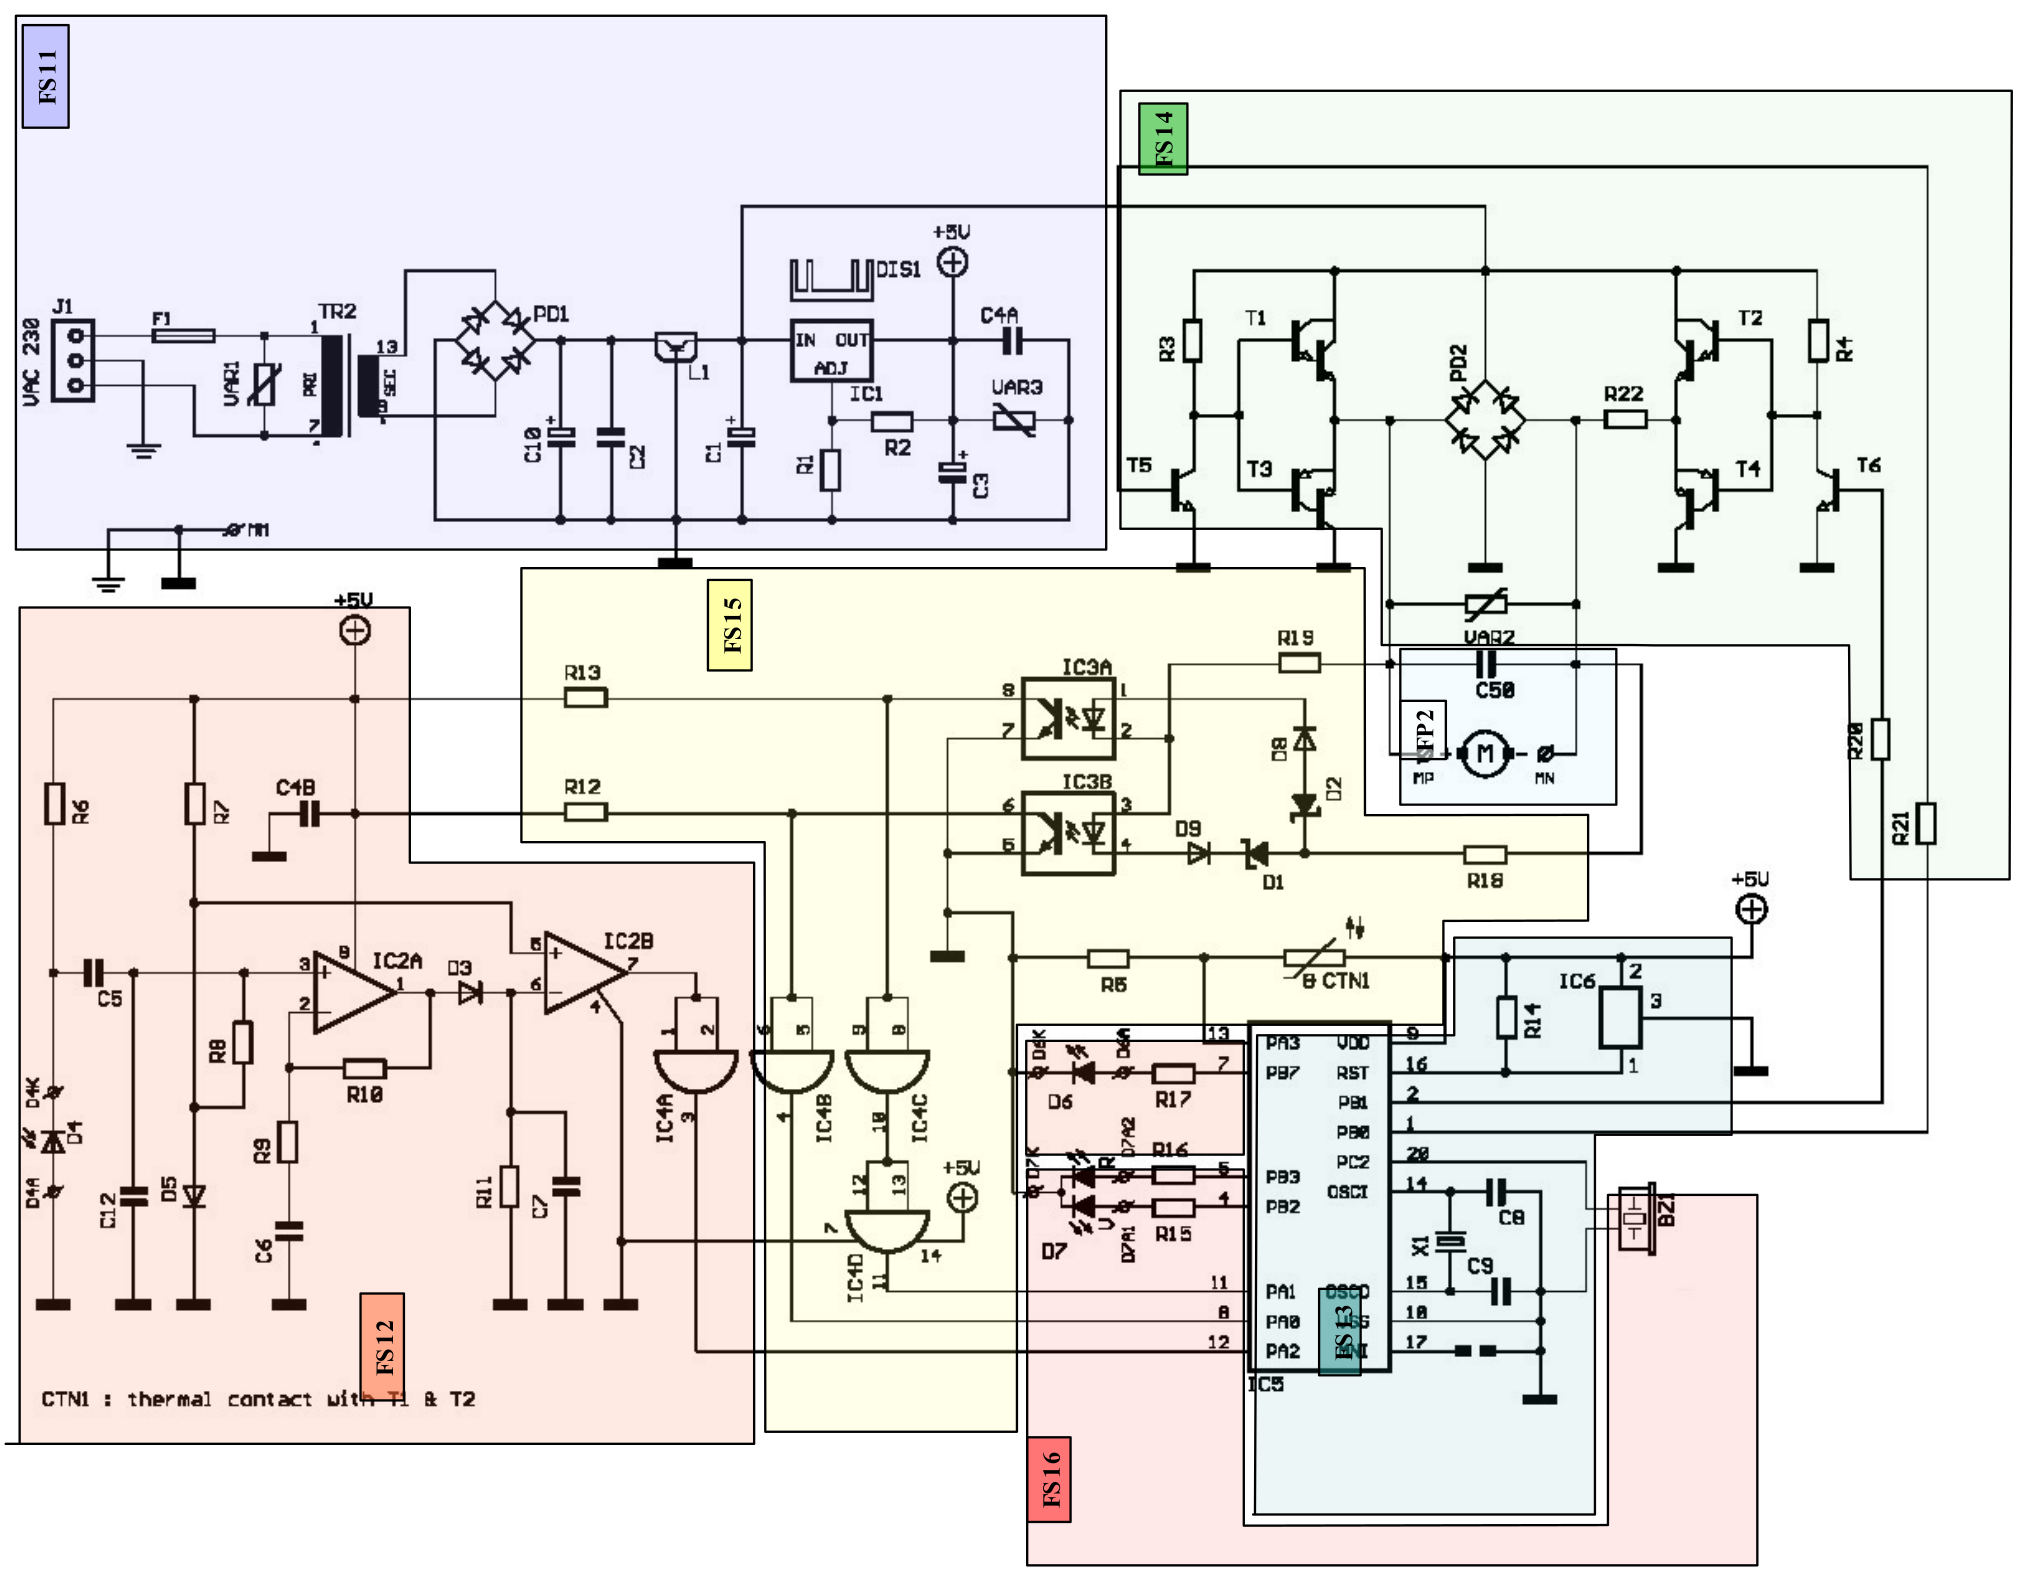
\includegraphics[width=\linewidth]{img/fonctionnel}
\caption{Schéma structurel du système}
\label{fig02}
\end{center}
\end{figure}


\question{Identifier sur le schéma structurel de la figure \ref{fig02} les structures qui correspondent aux blocs fonctionnels de la figure \ref{fig01}.}

\subsection{Le transformateur}

\question{Exprimer le rapport de transformation $r$ du transformateur. Calculer sa valeur.}

%\question{Donner la valeur maximale théorique du courant de sortie $I_S$ de TR1. En déduire la valeur maximale théorique du courant d'entrée $I_P$ de TR1.}

Le signal fourni par le secteur a une amplitude nominale de 230\,V et une fréquence de 50Hz . On connecte une charge résistive en sortie du transformateur.

\question{Représenter l'allure théorique de la tension de sortie du transformateur
$U_S = U_{AB}$.}

\subsection{Le pont de diodes}

On effectue un redressement de la tension abaissée à l'aide d'un pont de diodes. Les questions suivantes peuvent être traitées sur le schéma de la figure \ref{fig03}.

\begin{figure}[!ht]
\begin{center}
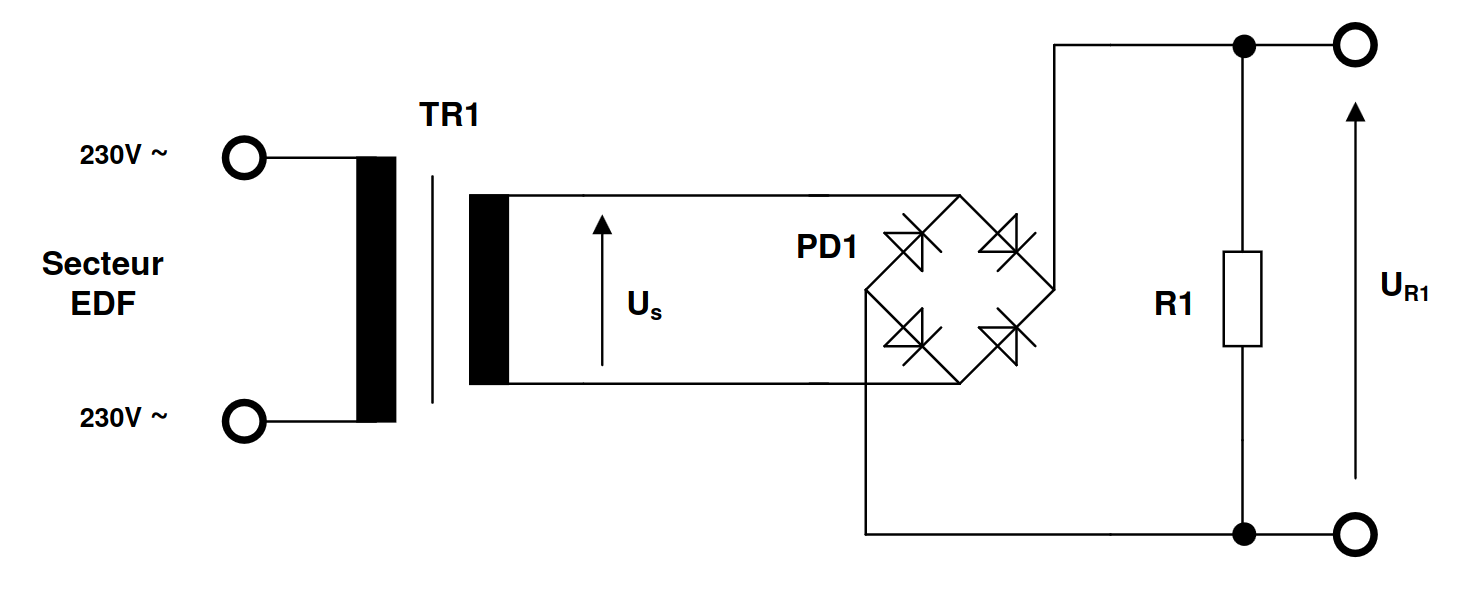
\includegraphics[width=\linewidth]{img/schema_1}
\caption{Schéma partiel de la chaîne d'adaptation}
\label{fig03}
\end{center}
\end{figure}

\question{Lors de l'alternance \textcolor{green!60!black}{\textbf{positive}} de $U_S$, flécher en \textcolor{green!60!black}{\textbf{vert}} le sens du courant qui traverse le pont de diodes et $R_1$.}

\question{Lors de l'alternance \textcolor{red}{\textbf{négative}} de $U_S$, flécher en \textcolor{red}{\textbf{rouge}} le sens du courant qui traverse le pont de diodes et $R_1$.}

\question{Que remarque-t-on pour le courant dans les 2 cas ? Que peut-on donc dire de $U_{R_1}$ ?}

\medskip
On supposera que les diodes du pont PD1 sont parfaites (pas de tension de seuil).

\question{Représenter $U_{R_1}$.}

\subsection{Le filtre}

Les condensateurs jouent le rôle de filtre qui lisse la tension.

\question{Représenter $U_{C_1}$.}

\section{Expérimentation}

Le schéma de la platine d'essais est donné à la figure \ref{fig04}. Les cavaliers JP1 à JP4 vont servir à étudier différentes configurations de montages. Les Points Tests PT1 à PT4 servent au branchement des appareils de mesures.

\begin{figure}[!ht]
\begin{center}
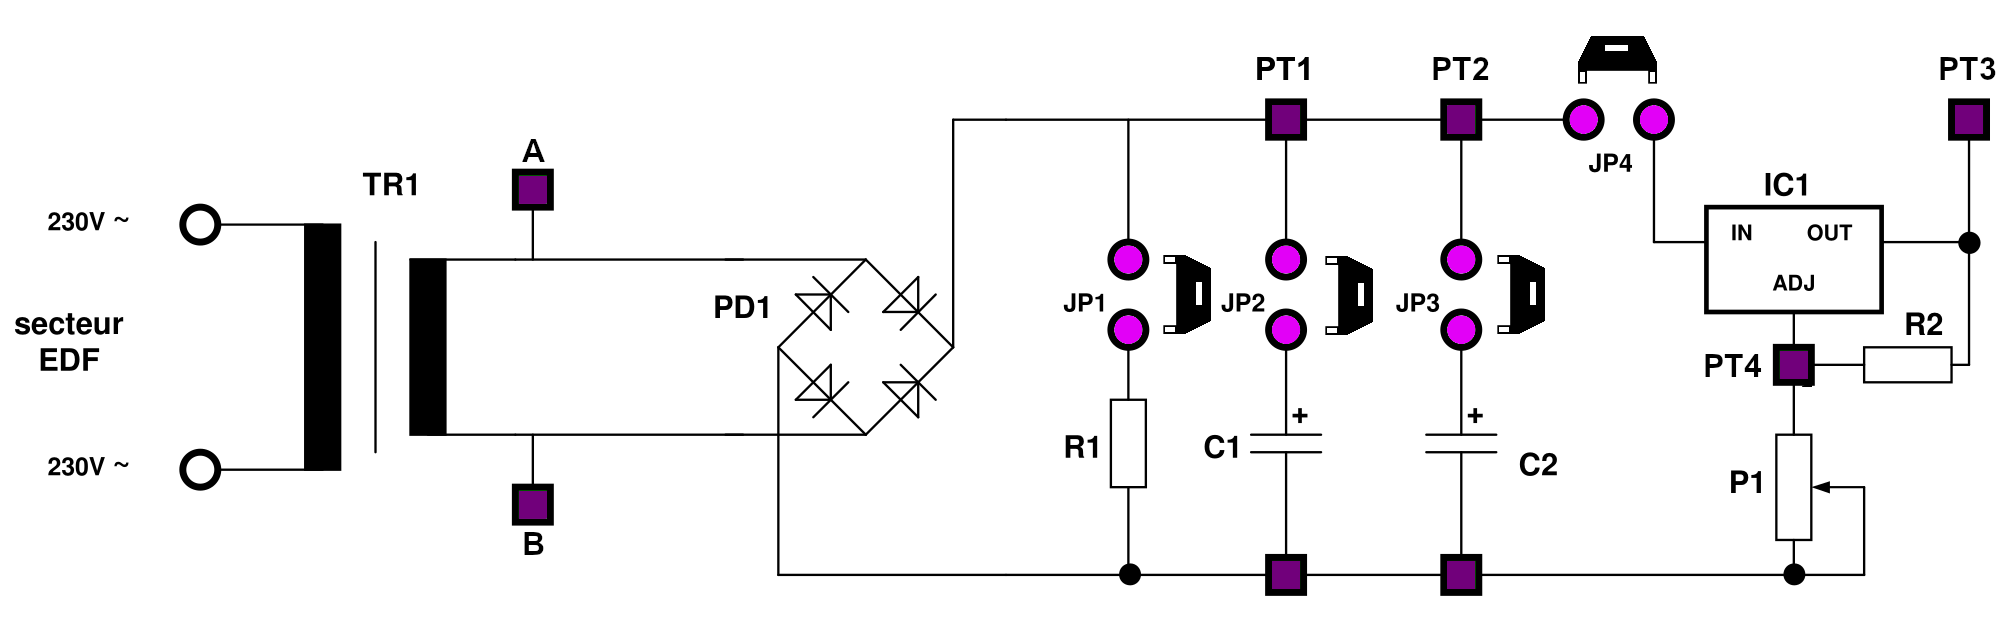
\includegraphics[width=\linewidth]{img/schema}
\caption{Schéma complet de la platine}
\label{fig04}
\end{center}
\end{figure}

\subsection{Mesures avec un transformateur à vide}

\textbf{Retirer tous les cavaliers de la platine d'essais. Brancher son cordon secteur.}

\question{Relever l'allure du signal $U_{AB}$ sur le \textbf{document-réponse 3}. Préciser sur le même relevé les différents calibres sélectionnés sur l'appareil de mesure.}

\question{Mesurer les valeurs maxi et mini de ce signal.}

\question{Proposer une méthode pour mesurer la valeur efficace de $U_{AB}$. Après validation par le professeur, effectuer cette mesure.}

\subsection{Le redressement sur charge résistive}

\textbf{Placer le cavalier JP1.}

\question{Relever l'allure du signal $U_{R_1}$ au point-test PT1 sur le \textbf{document-réponse 3}. Préciser sur le même relevé les différents calibres sélectionnés sur l'appareil de mesure.}

\question{Comparer avec $U_{R_1}$ dans la partie Préparation. Entourer sur le relevé une zone qui fait apparaître le seuil des diodes du pont.}

\question{Mesurer la valeur efficace de $U_{R_1}$.}

\question{Proposer une méthode pour mesurer la valeur moyenne de $U_{R_1}$. Après validation par le professeur, mesurer cette valeur.}

\subsection{Le filtrage}

\textbf{Laisser le cavalier JP1 en place. Placer le cavalier JP2.}

On effectue un filtrage avec $C_1 = 22\,\mu\text{F}$.

\question{ Relever l'allure du signal $U_{C_1}$ au point-test PT1. Préciser les différents calibres sélectionnés sur l'appareil de mesure.}

\question{Mesurer la valeur moyenne de ce signal.}

\question{Comparer avec la valeur moyenne de $U_{R_1}$.}

\medskip
\textbf{Laisser le cavalier JP1 en place. Enlever le cavalier JP2. Placer le cavalier JP3.}

On effectue ici un filtrage avec $C_2 = 220\,\mu\text{F}$.

\question{Relever l'allure du signal $U_{C_2}$ au point-test PT1. Préciser sur le même relevé les différents calibres sélectionnés sur l'appareil de mesure.}

\question{Mesurer la valeur moyenne de ce signal.}

\question{Comparer avec la valeur moyenne de $U_{C_1}$.}

\question{Conclure sur l'intérêt d'augmenter la valeur de la capacité de filtrage.}

\subsection{La régulation}

\textbf{Enlever le cavalier JP1. Laisser le cavalier JP3 en place. Placer le cavalier JP4.}

\question{Proposer une méthode pour mesurer la valeur $U_{\text{réf}}$. Après validation par le professeur, mesurer cette valeur.}

\question{Mesurer la tension de sortie du régulateur au point test PT3. Ajuster cette valeur à $5\,\text{V}$.}

\end{document}
